\chapter{Definite Integrals}

Integrals are a fundamental concept in calculus, which are used to
calculate areas, volumes, and many other things. A definite integral
calculates the net area between the function and the x-axis over a
given interval.

Recall that you can use a Riemann sum to estimate the area under a 
function, and that as we increase the number of subintervals, the 
estimated area approaches the actual area. In sigma notation we can 
express a Riemann sum as $$\sum_{i=1}^{n} f(x_i)\Delta x$$

\section{Definition}

The definite integral of a function $f(x)$ over an interval $[a, b]$
is defined as the limit of a Riemann sum as $n$ approaches $\infty$:

\begin{equation}
\int_{a}^{b} f(x) \, dx = \lim_{{n \to \infty}} \sum_{i=1}^{n} 
f(x_i^*) \Delta x
\end{equation}

where $x_i^*$ is a sample point in the $i^{th}$ subinterval of a
partition of $[a, b]$, $\Delta x = \frac{b-a}{n}$ is the width of each
subinterval, and the limit is taken as the number of subintervals $n$
approaches infinity.

\begin{Exercise}[label=defint1]
Express $$\lim_{n \to \infty} \sum_{i=1}^{n} (x_i^3 + x_i\sin{x_i})
\Delta x$$ as an integral on the interval $[0, \pi]$. 
\end{Exercise}

\begin{Answer}[ref=defint1]
Following the structure shown in the formal definition of a definite 
integral, we can set $f(x) = x^3 + x\sin{x}$ and re-write the limit of 
the sum as $\lim_{n \to \infty} \Sigma_{i=1}^{n} f(x)\Delta x = 
\int_{0}^{\pi} f(x)\,dx$. Therefore, the full definite integral 
would be written as $\int_{0}^{\pi} (x^3 + x\sin{x})\, dx$. 
\end{Answer}

\section{Positive and Negative Areas}
What if the function dips below the $x$-axis? We consider that area 
negative: that is, it represents a \textit{decrease} as opposed to 
an increase. Consider an oscillating object where $v(t) = 
\sin{\pi x}$ (figure \ref{fig:oscillate}). From $t = 0$ to $t = 1$, 
the velocity is positive, which means the object is moving 
\textit{away from} the starting position. The is a positive 
displacement. From $t = 1$ to $t = 2$, the velocity is negative. What 
does this tell you about the direction the object is moving and its 
displacement during this time period? A negative velocity means the 
object is moving \textit{back towards} the starting position, which 
implies a \textit{negative displacement}.

In general, areas above the $x$-axis are positive while areas below 
the $x$-axis are negative.

\begin{figure}
	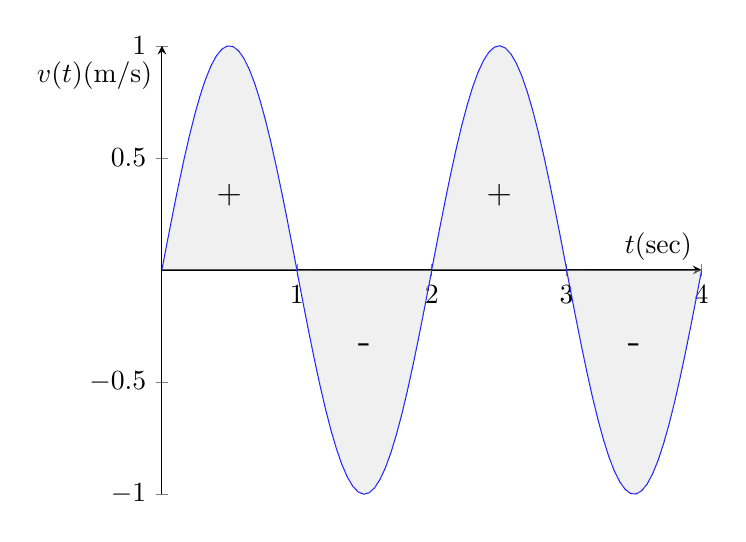
\begin{tikzpicture}
		\begin{axis}
		[xmin=0, xmax=4, ymin=-1, ymax=1, 
		xlabel=$t$(sec), ylabel=$v(t)$(m/s), 
		axis lines = center, ylabel style={yshift=-2.5ex,anchor=east}]
		\addplot[blue, samples=100, domain=0:4]{sin(pi*deg(x))};
        \fill [gray!30, opacity=0.4, domain=0:1, variable=\x]
      		(0, 0)
     		 -- plot ({\x}, {sin(pi*deg(\x))})
      		-- cycle;
      	\node[font=\large] at (0.5, 0.333) {+};
     	\fill [gray!30, opacity=0.4, domain=1:2, variable=\x]
      		(1, 0)
      		-- plot ({\x}, {sin(pi*deg(\x))})
      		-- cycle;
      	\node[font=\Large] at (1.5, -0.333) {-};
      	\fill [gray!30, opacity=0.4, domain=2:3, variable=\x]
      		(2, 0)
      		-- plot ({\x}, {sin(pi*deg(\x))})
      		-- cycle;
      	\node[font=\large] at (2.5, 0.333) {+};
      	\fill [gray!30, opacity=0.4, domain=3:4, variable=\x]
      		(3, 0)
      		-- plot ({\x}, {sin(pi*deg(\x))})
      		-- cycle;
      	\node[font=\Large] at (3.5, -0.333) {-};
		\end{axis}
	\end{tikzpicture}
	\caption{velocity of an oscillating object}
	\label{fig:oscillate}
\end{figure}

\section{Properties of Integrals}
The following properties of integrals apply when $f(x)$ is continuous 
or has a finite number of jump discontinuities on the interval $a 
\leq x \leq b$:
\begin{enumerate}
\item $$\int_{a}^{b} f(x)\,dx = - \int_{b}^{a} f(x)\,dx$$ 
%Property 1
\item If $a = b$, then $\Delta x = 0$ and therefore $$\int_{a}^{a} 
f(x)\,dx = 0$$%Property 2
\item $$\int_{a}^{b} c\,dx = c (b - a) \text{, where } c 
\text{ is any constant}$$%Property 3
\item $$\int_{a}^{b}[f(x) + g(x)]\,dx = \int_{a}^{b} f(x)\,dx + 
\int_{a}^{b} g(x)\,dx$$%Property 4
\item $$\int_{a}^{b} c f(x)\,dx = c \int_{a}^{b} f(x)\,dx
\text{, where } c \text{ is any constant}$$%Property 5
\item $$\int_{a}^{b}[f(x) - g(x)]\,dx = \int_{a}^{b} f(x)\,dx - 
\int_{a}^{b} g(x)\,dx$$%Property 6
\item $$\int_{a}^{c} f(x)\,dx + \int_{c}^{b} f(x)\,dx = 
\int_{a}^{b} f(x)\,dx \text{, where } a < c < b$$%Property 7
\item $$\text{If } f(x) \geq 0 \text{ for } a \leq x \leq b 
\text{, then } \int_{a}^{b} f(x)\,dx \geq 0$$%Property 8
\item $$\text{If } f(x) \geq g(x) \text{ for } a \leq x \leq b 
\text{, then} \int_{a}^{b} f(x)\,dx \geq \int_{a}^{b} g(x)\,dx$$
%Property 9
\item $$\text{If } m \leq f(x) \leq M \text{ for }a \leq x \leq b 
\text{, then } m (b - a) \leq \int_{a}^{b} f(x)\,dx \leq M (b - a)$$
%Property 10
\end{enumerate}


\section{Applications in Physics}
We've already seen that the area under a velocity function is 
displacement and the area under an acceleration function is change in 
velocity (Riemann Sums). We can use integrals to determine the change 
in position of an object over a given time frame. If we \textit{also} 
know the object's starting position, then we can state the object's 
ending position. Consider the graph of an object's velocity in figure 
\ref{fig:velocity}:

\begin{figure}[htbp]
	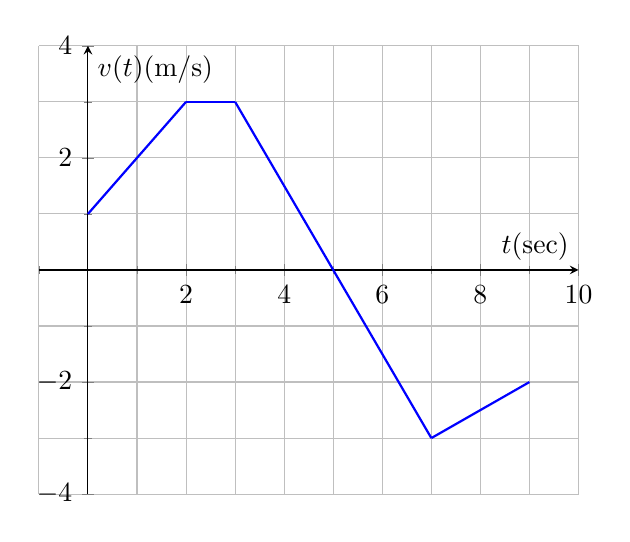
\begin{tikzpicture}
		\begin{axis}[axis lines = center, 
		xmin=-1, xmax=10, ymin=-4, ymax=4, 
		xlabel=$t$(sec), ylabel=$v(t)$(m/s), 
		xtick={}, ytick={}, grid=both, minor tick num = 1]
		\addplot[blue, thick] coordinates {(0, 1) (2, 3)};
		\addplot[blue, thick] coordinates {(2, 3) (3, 3)};
		\addplot[blue, thick] coordinates {(3, 3) (7, -3)};
		\addplot[blue, thick] coordinates {(7, -3) (9, -2)};
		\end{axis}
	\end{tikzpicture}
	\caption{Velocity of an object from $t=0$ to $t=9$}
	\label{fig:velocity}
\end{figure}

We can determine the net displacement of the object from $t = 0$ to 
$t = 9$ by evaluating $\int_{0}^{9} v(t) \ , dt$. Since the definite 
integral is equal to the area under the curve, we need to find the 
total area. As the function consists of straight lines, we will leave 
the explicit calculation of the area as an exercise for the student. 
You should find that the total positive area (above the $x$-axis) is 
10 meters and the total negative area (below the $x$-axis) is 8 meters. 
Therefore, the object's displacement over the specified time interval 
is $10 - 8 = 2$ meters. 

When you push on something to move it, you are applying a force over 
a distance (assuming you are strong enough to move it!). The integral 
of force as a function of distance is the \textit{work} done on that 
object.  Work is the change in kinetic energy (KE) of an object. 
Mathematically, this is $$\int_{a}^{b} F(d)\,dd = \Delta KE = 
\frac{1}{2} m (v_f^2 - v_i^2)$$

If you integrate the force as a function of time, that is 
\textit{impulse}. Impulse is the change in momentum (p) of the 
object. Mathematically, this is $$\int_{a}^{b} F(t)\,dt = \Delta p 
= m (v_f - v_i)$$

Example problem: You push a 3 kg box with force $F(d) = 0.5d$, where 
$d$ is measured in meters and $F$ is measured in Newtons. If the box 
was initially at rest, what is its speed when it reaches the 2 meter 
mark? (Hint: $KE = \frac{1}{2} m v^2$.) 

Solution: Change in kinetic energy is the area under a force-distance 
curve. We can plot the force applied to the box from d=0 to d=2 (see 
figure \ref{fig:KEbox}):

\begin{figure}[htbp]
	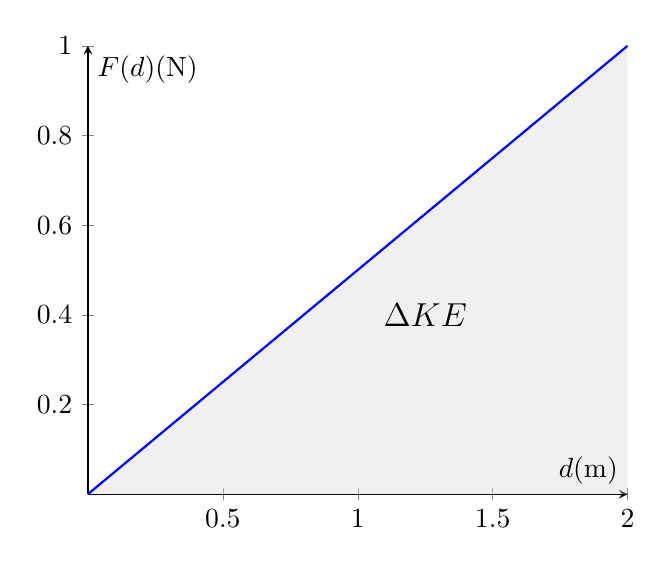
\begin{tikzpicture}
		\begin{axis}
		[xmin=0, xmax=2, ymin=0, ymax=1, 
		xlabel=$d$(m), ylabel=$F(d)$(N), axis lines = center]
            \fill[gray!30, opacity=0.4](0,0) --(2, 0) -- (2,1) -- cycle;
            \node[font=\large] at (1.25, 0.4) {$\Delta KE$};
		\addplot[blue, thick]{0.5*x};
		\end{axis}
	\end{tikzpicture}
 \caption{Force applied to a box over a distance; the shaded area 
 represents the change in kinetic energy.}
 \label{fig:KEbox}
\end{figure}

Given that the box's initial velocity is $0 \frac{m}{s}$, we know that 
the initial kinetic energy (KE) is $0J$. This implies that $KE_f = 
\Delta KE$. We can find $\Delta KE$ from the shaded area:\\
$$\Delta KE = \frac{1}{2} (2m) (1N) = 1 J = KE_f$$\\
Solving for the final velocity:\\
$$KE_f = 1 J = \frac{1}{2}(3kg)(v^2)$$
$$2 J = (3 kg) (v^2)$$
$$\frac{2}{3} \frac{m^2}{s^2} = v^2$$
$$v=\sqrt{\frac{2}{3} \frac{m^2}{s^2}} \approx 0.816 \frac{m}{s}$$


\section{Applications in Mathematics}
%length of curves/arc length explanation

\begin{Exercise}[label=length1]
Write an integral that gives the length of the requested curve.
	\begin{enumerate}
	\item $y = \ln{x}$ from $x = 1$ to $x = 3$
	\item $y = \sin{x}$ from $x = 0$ to $x = \pi$
	\item $y = \frac{x^3}{3} + \frac{1}{4x}$ from $x = 1$ to $x = 4$
	\item $y = \ln{\cos{x}}$ from $x = 0$ to $x = \frac{\pi}{3}$
	\end{enumerate}	 
\end{Exercise}

\begin{Answer}[ref=length1]
	\begin{enumerate}
	\item $L = \int_{1}^{3} \sqrt{1 + \frac{1}{x^2}}\,dx$
	\item $L = \int_{0}^{\pi} \sqrt{1 + \cos^2{x}}\,dx$
	\item $L = \int_{1}^{4} \sqrt{1 + (x^2-\frac{1}{4x^2})^2}\,dx$
	\item $L = \int_{0}^{\frac{\pi}{3}} \sqrt{1 + (\frac{1}{\cos{x}} 
	\times - \sin{x})^2}\,dx = \int_{0}^{\frac{\pi}{3}} \sqrt{1 + 
	\tan^2{x}}\,dx$
	\end{enumerate}
\end{Answer}


\section{Practice Exercises}
\begin{Exercise}[label=defint2]
Given that $\int_{0}^{1} x^2\,dx = \frac{1}{3}$, use the properties 
of integrals to evaluate $\int_{0}^{1} (5-6x^2)\,dx$. 
\end{Exercise}

\begin{Answer}[ref=defint2]
By property 6, we know that $$\int_{0}^{1} (5-6x^2)\,dx = \int_{0}^{1} 
5\,dx - \int_{0}^{1} 6x^2\,dx$$\\
By property 5, we know that $$\int_{0}^{1} 5\,dx - \int_{0}^{1} 6x^2\,
dx = \int_{0}^{1} 5\,dx - 6\int_{0}^{1} x^2\,dx$$\\
By property 3, we know that $$\int_{0}^{1} 5\,dx = 5(1 - 0) = 5$$\\
Putting it all together, we see that $$\int_{0}^{1} (5-6x^2)\,dx = 5 
- 6(\frac{1}{3}) = 5 - 2 = 3$$
\end{Answer}

\begin{Exercise}[label=defint3]
	This question was originally presented as a multiple-choice problem 
	on the 2012 AP Calculus BC exam. The graph of $f$ is shown. What is 
	the value of $\int_{0}^{4} f(x)\,dx$?\\
	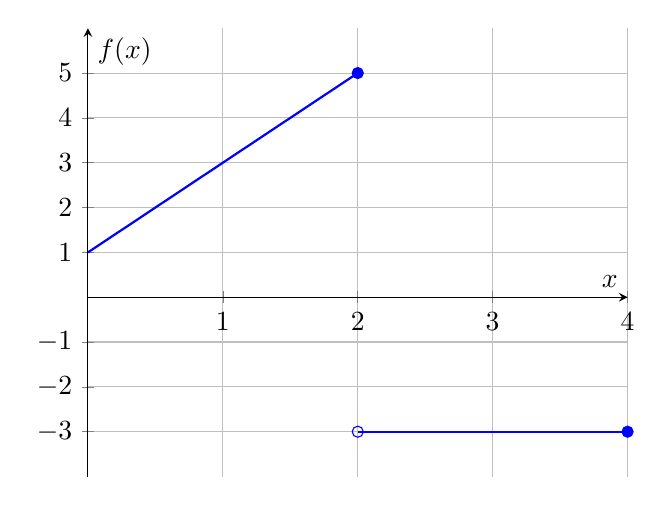
\begin{tikzpicture}
		\begin{axis}
		[xmin=0, xmax=4, xlabel=$x$, 
		ylabel=$f(x)$, ymin = -4, ymax=6, 
		axis lines = center, minor tick = 1, grid = major, 
		ytick={-3, -2, -1, 1, 2, 3, 4, 5}]
		      \addplot[blue, thick]coordinates{(0, 1) (2, 5)};
		      \addplot[mark=*, blue]coordinates{(2, 5)};
		      \addplot[mark=o, blue]coordinates{(2, -3)};
		      \addplot[blue, thick]coordinates{(2, -3) (4, -3)};
    		\addplot[mark=*, blue]coordinates{(4, -3)};
		\end{axis}
	\end{tikzpicture}
\end{Exercise}

\begin{Answer}[ref=defint3]
We can break the integral into two parts: from $x = 0$ to $x = 2$ 
(shaded in blue), and from $x = 2$ to $x = 4$ (shaded in red). The 
blue portion is a trapezoid and so has a total area of $\frac{1}{2} 
(b_1 + b_2) (h) = \frac{1}{2} (1 + 5) (2) = 6$. Because it is above 
the $x$-axis, the area is positive. The red portion is a rectangle and 
has a total area of $2 \times 3 = 6$ and is \textit{negative} because 
it lies below the $x$-axis. Therefore, the total area is $6 + -6 = 0$. \\

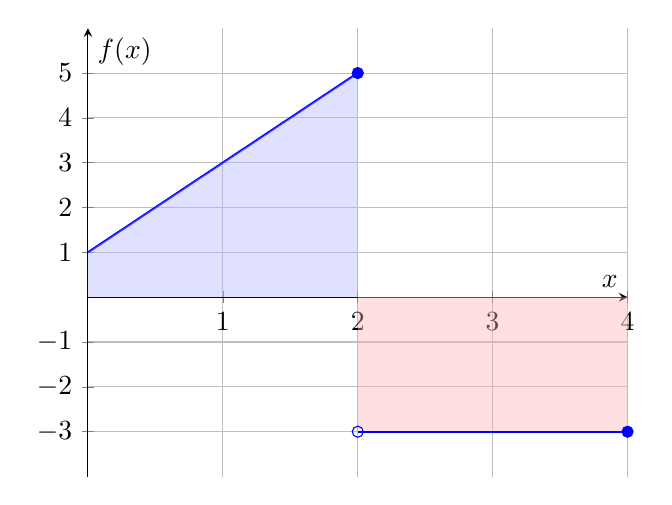
\begin{tikzpicture}
		\begin{axis}
		[xmin=0, xmax=4, xlabel=$x$, 
		ylabel=$f(x)$, ymin = -4, ymax=6, 
		axis lines = center, minor tick = 1, grid = major, 
		ytick={-3, -2, -1, 1, 2, 3, 4, 5}]
		      \addplot[blue, thick]coordinates{(0, 1) (2, 5)};
		      \fill[blue!30, opacity=0.4](0, 0)--(2, 0)--(2, 5)--(0,1)--cycle;
		      \fill[red!30, opacity=0.4](2, 0) rectangle (4, -3);
		      \addplot[mark=*, blue]coordinates{(2, 5)};
		      \addplot[mark=o, blue]coordinates{(2, -3)};
		      \addplot[blue, thick]coordinates{(2, -3) (4, -3)};
    		\addplot[mark=*, blue]coordinates{(4, -3)};
		\end{axis}
	\end{tikzpicture}
\end{Answer}

\begin{Exercise}[label=defint4]
	This question was originally presented as a multiple-choice problem 
	on the 2012 AP Calculus BC exam. The graph of the piecewise function 
	$g(x)$ is shown. What is the value of $\int_{-1}^{9} 3 g(x) + 2\,dx$?
	
	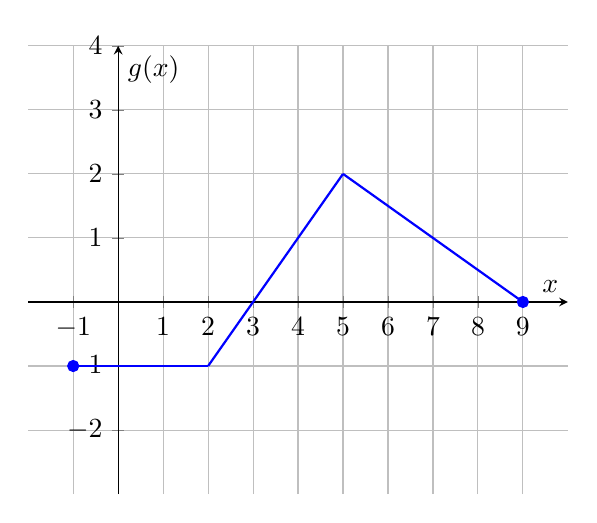
\begin{tikzpicture}
		\begin{axis}
		[xmin=-2, xmax=10, ymin=-3, ymax=4, 
		axis lines = center, xlabel=$x$, ylabel=$g(x)$, 
		grid=major, ytick={-2, -1, 1, 2, 3, 4}, xtick={-1, 1, 2, 3, 4, 5, 6, 7, 8, 9}]
		\addplot[blue, thick]coordinates{(-1, -1) (2, -1)};
		\addplot[blue, thick]coordinates{(2, -1) (5, 2)};
		\addplot[blue, thick]coordinates{(5, 2) (9, 0)};
            \addplot[blue, mark=*, only marks]coordinates{(-1, -1) (9, 0)};
		\end{axis}
	\end{tikzpicture}
\end{Exercise}

\begin{Answer}[ref=defint4]
Using the properties of integrals, we can rewrite $\int_{-1}^{9} 3 
g(x) + 2\,dx$ as $3 \int_{-1}^{9} g(x)\,dx + 2 (9-(-1))$. From the 
graph, we can determine $\int_{-1}^{9} g(x)\,dx = 2.5$. Therefore, 
$\int_{-1}^{9} 3 g(x) + 2\,dx = 3 (2.5) + 2 (10) = 27.5$. 
\end{Answer}

\begin{Exercise}[label=defint5]
The arc length function for a curve $f(x)$, where $f$ is an increasing 
function, is given by $s(x) = \int_{0}^{x} \sqrt{3t + 5}\,dt$. If $f$ 
has $y$-intercept 2, find an equation for $f$. What point on $f$ is 
three units from the $y$-intercept? Give your answer to the thousandths 
place. 
\end{Exercise}

\begin{Answer}[ref=defint5]
From looking at the structure of the given arc length integral, we can 
see that $f'(x) = \sqrt{3x + 4}$. Taking the antiderivative, we find 
that $f(x) = \frac{2}{9}(3x + 4)^{3 / 2} + C$. Substituting $f(0) = 2$
, we can solve for $C$. $$2 = \frac{2}{9}(3(0) + 4)^{3 / 2} + C$$ 
$$2 = \frac{2}{9}(4)^{3 / 2} + C$$ 
$$2 = \frac{2}{9}(2)^3 + C$$ 
$$2 = \frac{16}{9} + C$$ 
$$\frac{18}{9} = \frac{16 + 9C}{9}$$ 
$$18 = 16 + 9C$$ 
$$2 = 9C$$ 
$$C = \frac{2}{9}$$\\ 
Therefore, $f(x) = \frac{2}{3}(3x + 4)^{3 / 2} + \frac{2}{9}$. To find 
the coordinate point where $s(x) = 3$, we first note that the 
antiderivative of $\sqrt{3t + 5}$ is $\frac{2}{9}(3t + 5)^{3 / 2} + C$. 
Therefore, $s(x) = \frac{2}{9}(3x + 5)^{3 / 2} - \frac{2}{9}(5)^{3 / 2}$. 
Setting $s(x) = 3$ and solving for $x$, we find that $x = 1.159$
\end{Answer}